 \documentclass[pdftex,12pt, oneside]{article}

%\usepackage[paperwidth=8.5in, paperheight=13in]{geometry} % Folio
\usepackage[paperwidth=8.27in, paperheight=11.69in]{geometry} % A4

\usepackage{makeidx}         % allows index generation
\usepackage{graphicx}        % standard LaTeX graphics tool
                             % when including figure files
\usepackage[bottom]{footmisc}% places footnotes at page bottom
\usepackage[english]{babel}
\usepackage{enumerate}
\usepackage{paralist}
\usepackage{float}
\usepackage{gensymb}  
\usepackage{listings}
\usepackage{color}
\usepackage{mathtools} % atau \usepackage{amsmath}
\renewcommand{\baselinestretch}{1.5}

\newcommand{\HRule}{\rule{\linewidth}{0.5mm}}

\definecolor{codegreen}{rgb}{0,0.6,0}
\definecolor{codegray}{rgb}{0.5,0.5,0.5}
\definecolor{codepurple}{rgb}{0.58,0,0.82}
\definecolor{backcolor}{rgb}{0.95,0.95,0.92}

\lstdefinestyle{mystyle}{
  backgroundcolor=\color{backcolor},
  commentstyle=\color{codegreen},
  keywordstyle=\color{magenta},
  stringstyle=\color{codepurple},
  basicstyle=\footnotesize,
  breakatwhitespace=false,
  breaklines=true,
  captionpos=b,
  keepspaces=true,
  numbers=left,
  numbersep=5pt,
  showspaces=false,
  showstringspaces=false,
  showtabs=false,
  tabsize=2
}

\lstset{style=mystyle}


\begin{document}
\sloppy % biar section ga melebar melewati kertas

\begin{center}
{\large IMPLEMENTASI RANCANGAN SISTEM BASIS DATA - WS PBB}
\\[1cm]
XX April 2017\\
Priyanto Tamami, S.Kom.
\end{center}

%\frontmatter%%%%%%%%%%%%%%%%%%%%%%%%%%%%%%%%%%%%%%%%%%%%%%%%%%%%%%


%%%%%%%%%%%%%%%%%%%%%%%%%%%%%%%%%%%%%%%%%%%%%%%%%%%%%%%%%%%%%%%%%%%%%%

\section{TAHAPAN IMPLEMENTASI}

Tahapan implementasi dari sistem basis data untuk aplikasi \textit{Web Service} PBB adalah sebagai berikut :

\begin{enumerate}[1.]
  \item Telaah Ulang Rancangan Sistem Basis Data
  \item Penjadwalan Tugas Pengembangan Sistem Basis Data
  \item \textit{Coding} Program
  \item Pengujian Sistem Basis Data
\end{enumerate}

Tahapan secara rinci akan dijelaskan sebagai berikut.

\subsection{Telaah Ulang Rancangan}

Penelaahan ulang dilakukan melalui alur data yang terjadi pada saat aplikasi digunakan nantinya. Kebutuhan akan sistem basis data dapat ditelaah berdasarkan diagram \textit{use-case} seperti pada gambar \ref{fig:use-case} :

\begin{figure}[H]
	\centering
	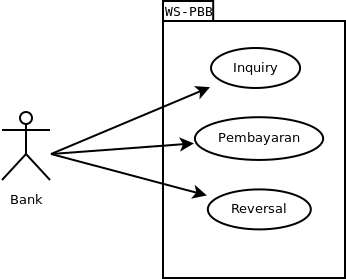
\includegraphics[width=0.5\textwidth]{./resources/001-uml-use-case}
	\caption{Diagram \textit{Use-Case}}
	\label{fig:use-case}
\end{figure}

Pada diagram tersebut, aplikasi nantinya akan melayani 3 (tiga) hal, yaitu \textit{inquiry}, pencatatan pembayaran, dan \textit{reversal} pembayaran. Kebutuhan rinci untuk tiap aktivitas tersebut adalah sebagai berikut :

\begin{enumerate}[1.]
	\item \textit{Inquiry} Data
	
	Pada aktivitas \textit{inquiry} data, tabel yang dibutuhkan adalah tabel SPPT sebagai tabel utama yang memuat informasi nama wajib pajak, tahun pajak, dan besarnya PBB-P2 terhutang. Tabel lain yang diperlukan adalah tabel REF\_KECAMATAN dan REF\_KELURAHAN yang menyimpan informasi nama Kecamatan dan nama Desa/Kelurahan. 
	
	\item Pencatatan Pembayaran
	
	Pada aktivitas pencatatan pembayaran SPPT PBB-P2, tabel yang dibutuhkan atau digunakan adalah sebagai berikut :
	
	\begin{itemize}
		\item Tabel SPPT sebagai tabel yang menyimpan informasi utama dari tagihan tahun pajak tertentu, nantinya \textit{field} STATUS\_PEMBAYARAN\_SPPT pada tabel ini akan diubah menjadi 1 (satu) apabila proses pencatatan pembayaran berhasil.
		\item Tabel PEMBAYARAN\_SPPT digunakan sebagai tempat untuk mencatatkan transaksi pembayaran sesuai aplikasi SISMIOP. 
		\item Tabel DAT\_OP\_BUMI digunakan untuk mengambil informasi kode zona nilai tanah dan nilai sistem bumi (tanah) sebagai bahan penyusunan kode Nomor Transaksi Pajak Daerah (NTPD).
		\item Tabel REF\_KECAMATAN dan REF\_KELURAHAN yang digunakan untuk menampilkan informasi nama Kecamatan dan nama Desa/Kelurahan sebagai bahan informasi pencetakan Surat Setoran Pajak Daerah oleh pihak Bank / Tempat Pembayaran.
		\item Tabel LOG\_TRX\_PEMBAYARAN yang digunakan sebagai tempat penyimpanan aktivitas pencatatan transaksi yang telah terjadi.
	\end{itemize} 
	
	\item \textit{Reversal} Pembayaran
	
	Pada aktivitas \textit{reversal} pembayaran SPPT PBB-P2, dimaksudkan apabila ada kesalahan pencatatan pembayaran yang telah terjadi sebelumnya, tagihannya dapat dikembalikan ke status terhutang kembali. Adapun tabel yang digunakan untuk aktivitas ini adalah sebagai berikut :
	
	\begin{itemize}
		\item Tabel SPPT, tabel ini digunakan agar aplikasi dapat mengubah / memperbarui \textit{field} STATUS\_PEMBAYARAN\_SPPT menjadi 0 (nol) yang artinya Nomor Objek Pajak (NOP) untuk tahun pajak tercantum belum dibayarkan dan dalam status terhutang.
		\item Tabel PEMBAYARAN\_SPPT, tabel ini digunakan agar aplikasi dapat menghapus data terakhir saat terjadinya pembayaran.
		\item Tabel LOG\_TRX\_PEMBAYARAN, tabel ini digunakan oleh aplikasi untuk melakukan pencocokan data Nomor Transaksi Pajak Daerah (NTPD) yang menunjukkan bahwa transaksi yang akan dilakukan \textit{reversal} adalah transaksi yang pernah dilakukan pencatatan pembayaran sebelumnya.
		\item Tabel LOG\_REVERSAL, tabel ini digunakan oleh aplikasi untuk menyimpan catatan aktivitas \textit{reversal} yang telah terjadi.
	\end{itemize}
\end{enumerate}

\subsection{Penjadwalan tugas pengembangan}

Jadwal tugas pengembangan untuk membangun sistem basis data pada aplikasi \textit{Web Service} dilakukan oleh 1 (satu) orang fungsional Pranata Komputer dan dapat diselesaikan dalam 1 hari saja karena struktur tabel pada basis data sebagian menggunakan sistem yang sudah ada (dari SISMIOP), sehingga hanya diperlukan tabel LOG\_REVERSAL dan tabel LOG\_TRX\_PEMBAYARAN saja. Adapun \textit{store procedures} yang dibangun juga cukup sederhana.

\subsection{Coding Program (Pembuatan database, tabel, relasi tabel, indeks, dan trigger)}

Bagian \textit{coding} program akan terdiri dari beberapa hal, yaitu :

\begin{enumerate}[1.]
	\item Pembuatan Database
	\item Pembuatan Tabel
	\item Pembuatan Relasi Tabel
	\item Pembuatan Indeks
	\item Pembuatan \textit{Trigger}
	\item Pembuatan \textit{Store Procedure}
\end{enumerate}

\subsection{menguji database}

\subsection{pelatihan pengguna - ops}


\section{RANCANGAN}

% terlampir dari kegiatan III.D.1

\section{LOKASI}

\section{SKEMA DAN KAMUS}

\section{BESARAN}

\section{JENIS DBMS}

\section{JENIS APLIKASI YANG MENGGUNAKAN DB}

\end{document}